\documentclass{article}
\usepackage{listings}
\usepackage{xcolor}
\usepackage[margin=1in]{geometry}
\usepackage{amsmath}
\usepackage{amssymb}
\usepackage{fancyhdr}
\usepackage{blindtext}
\usepackage{titling}
\usepackage{siunitx}
\usepackage{hyperref}
\usepackage{graphicx}
\usepackage{environ}
\usepackage{cite}
\usepackage[square,numbers]{natbib}

\graphicspath{{./images/}}

\NewEnviron{eq}{
\begin{equation*}\begin{split}
  \BODY
\end{split}\end{equation*}
}

\NewEnviron{mhp}{
    \begin{minipage}{0.5\textwidth}
        \BODY
    \end{minipage}
}

\author{.}
\title{.}
\date{\today}

\newcolumntype{L}[1]{>{\raggedright\let\newline\\\arraybackslash\hspace{0pt}}m{#1}}

\pagestyle{fancy}
\setlength{\droptitle}{-10em}
\renewcommand{\headrulewidth}{0pt}
\renewcommand{\footrulewidth}{0pt}
\renewcommand\maketitlehookb{\centering COSC1047N}
\renewcommand\maketitlehookc{\centering 219645940}

\newcommand{\m}[1]{\texttt{#1}}
\newcommand{\bn}[1]{\m{0b#1}}
\newcommand{\hx}[1]{\m{0x#1}}
\newcommand{\hem}{\hspace{1em}}
\newcommand{\vem}{\vpsace{1em}}
\newcommand{\pgrph}[1]{\paragraph{#1}\mbox{}\\\\}

\fancyhf{}
\rhead{Solar System Sim}
\rfoot{Page \thepage}

\definecolor{codegreen}{rgb}{0,0.6,0}
\definecolor{codegray}{rgb}{0.5,0.5,0.5}
\definecolor{codepurple}{rgb}{0.58,0,0.82}
\definecolor{backcolour}{rgb}{0.90,0.90,0.90}
\definecolor{shellcolor}{rgb}{0.1,0.5,0.2}

\lstdefinestyle{codestyle}{
    backgroundcolor=\color{backcolour},
    commentstyle=\color{codegreen},
    keywordstyle=\color{magenta},
    numberstyle=\tiny\color{codegray},
    stringstyle=\color{codepurple},
    basicstyle=\ttfamily\footnotesize,
    breakatwhitespace=false,
    breaklines=true,
    captionpos=b,
    keepspaces=true,
    numbers=left,
    numbersep=5pt,
    showspaces=false,
    showstringspaces=false,
    showtabs=false,
    tabsize=2
}

\lstdefinestyle{termstyle}{
    backgroundcolor=\color{backcolour},
    commentstyle=\color{codegreen},
    keywordstyle=\color{magenta},
    numberstyle=\tiny\color{codegray},
    stringstyle=\color{codepurple},
    basicstyle=\ttfamily\footnotesize,
    breakatwhitespace=false,
    breaklines=true,
    captionpos=b,
    keepspaces=true,
    showspaces=false,
    showstringspaces=false,
    showtabs=false,
    tabsize=2,
    moredelim=**[is][\color{cyan}]{@}{@},
    moredelim=**[is][\color{shellcolor}]{!}{!}
}

\newcommand\mycite[2]{(\citealt[#2]{#1})}

\begin{document}
    \begin{titlepage}
        \begin{center}
            \topskip0pt
            \vspace*{\fill}

            \Huge
            \textbf{Solar System Sim}

            \vspace{0.5cm}
            \Large
            A VR solar system simulation.

            \vspace{1.5cm}

            \textbf{Jacob Burtch, Max Mcnally, Chelaka Fernando, Marizza Ranasinghe, Braeden Hong}

            \Large
            Dr. Miguel Garcia-Ruiz\\
            Algoma University\\
            Faculty of Computer Science and Technology\\
            COSC4426\\
            Sault Ste. Marie, Ontario, Canada\\
            \today
            \vspace*{\fill}
        \end{center}
    \end{titlepage}
    \newpage
    \section{The Simulation}
    This project features a VR simulation of the solar system. This simulation includes all of the main components of the solar system. Namely, the sun and the planets. The simulation also features the Earth's moon, but not the moons of all the other planets. Other objects such as asteroids are simulated as well. The application simulates the solar system with a custom gravity simulation to more accurately simulate planetary orbits. Figure \ref{initialvr} shows the first test of the VR system in the program showing the two controller rays that show where the VR controllers are in the world.
    \begin{figure}[h]
        \centering
        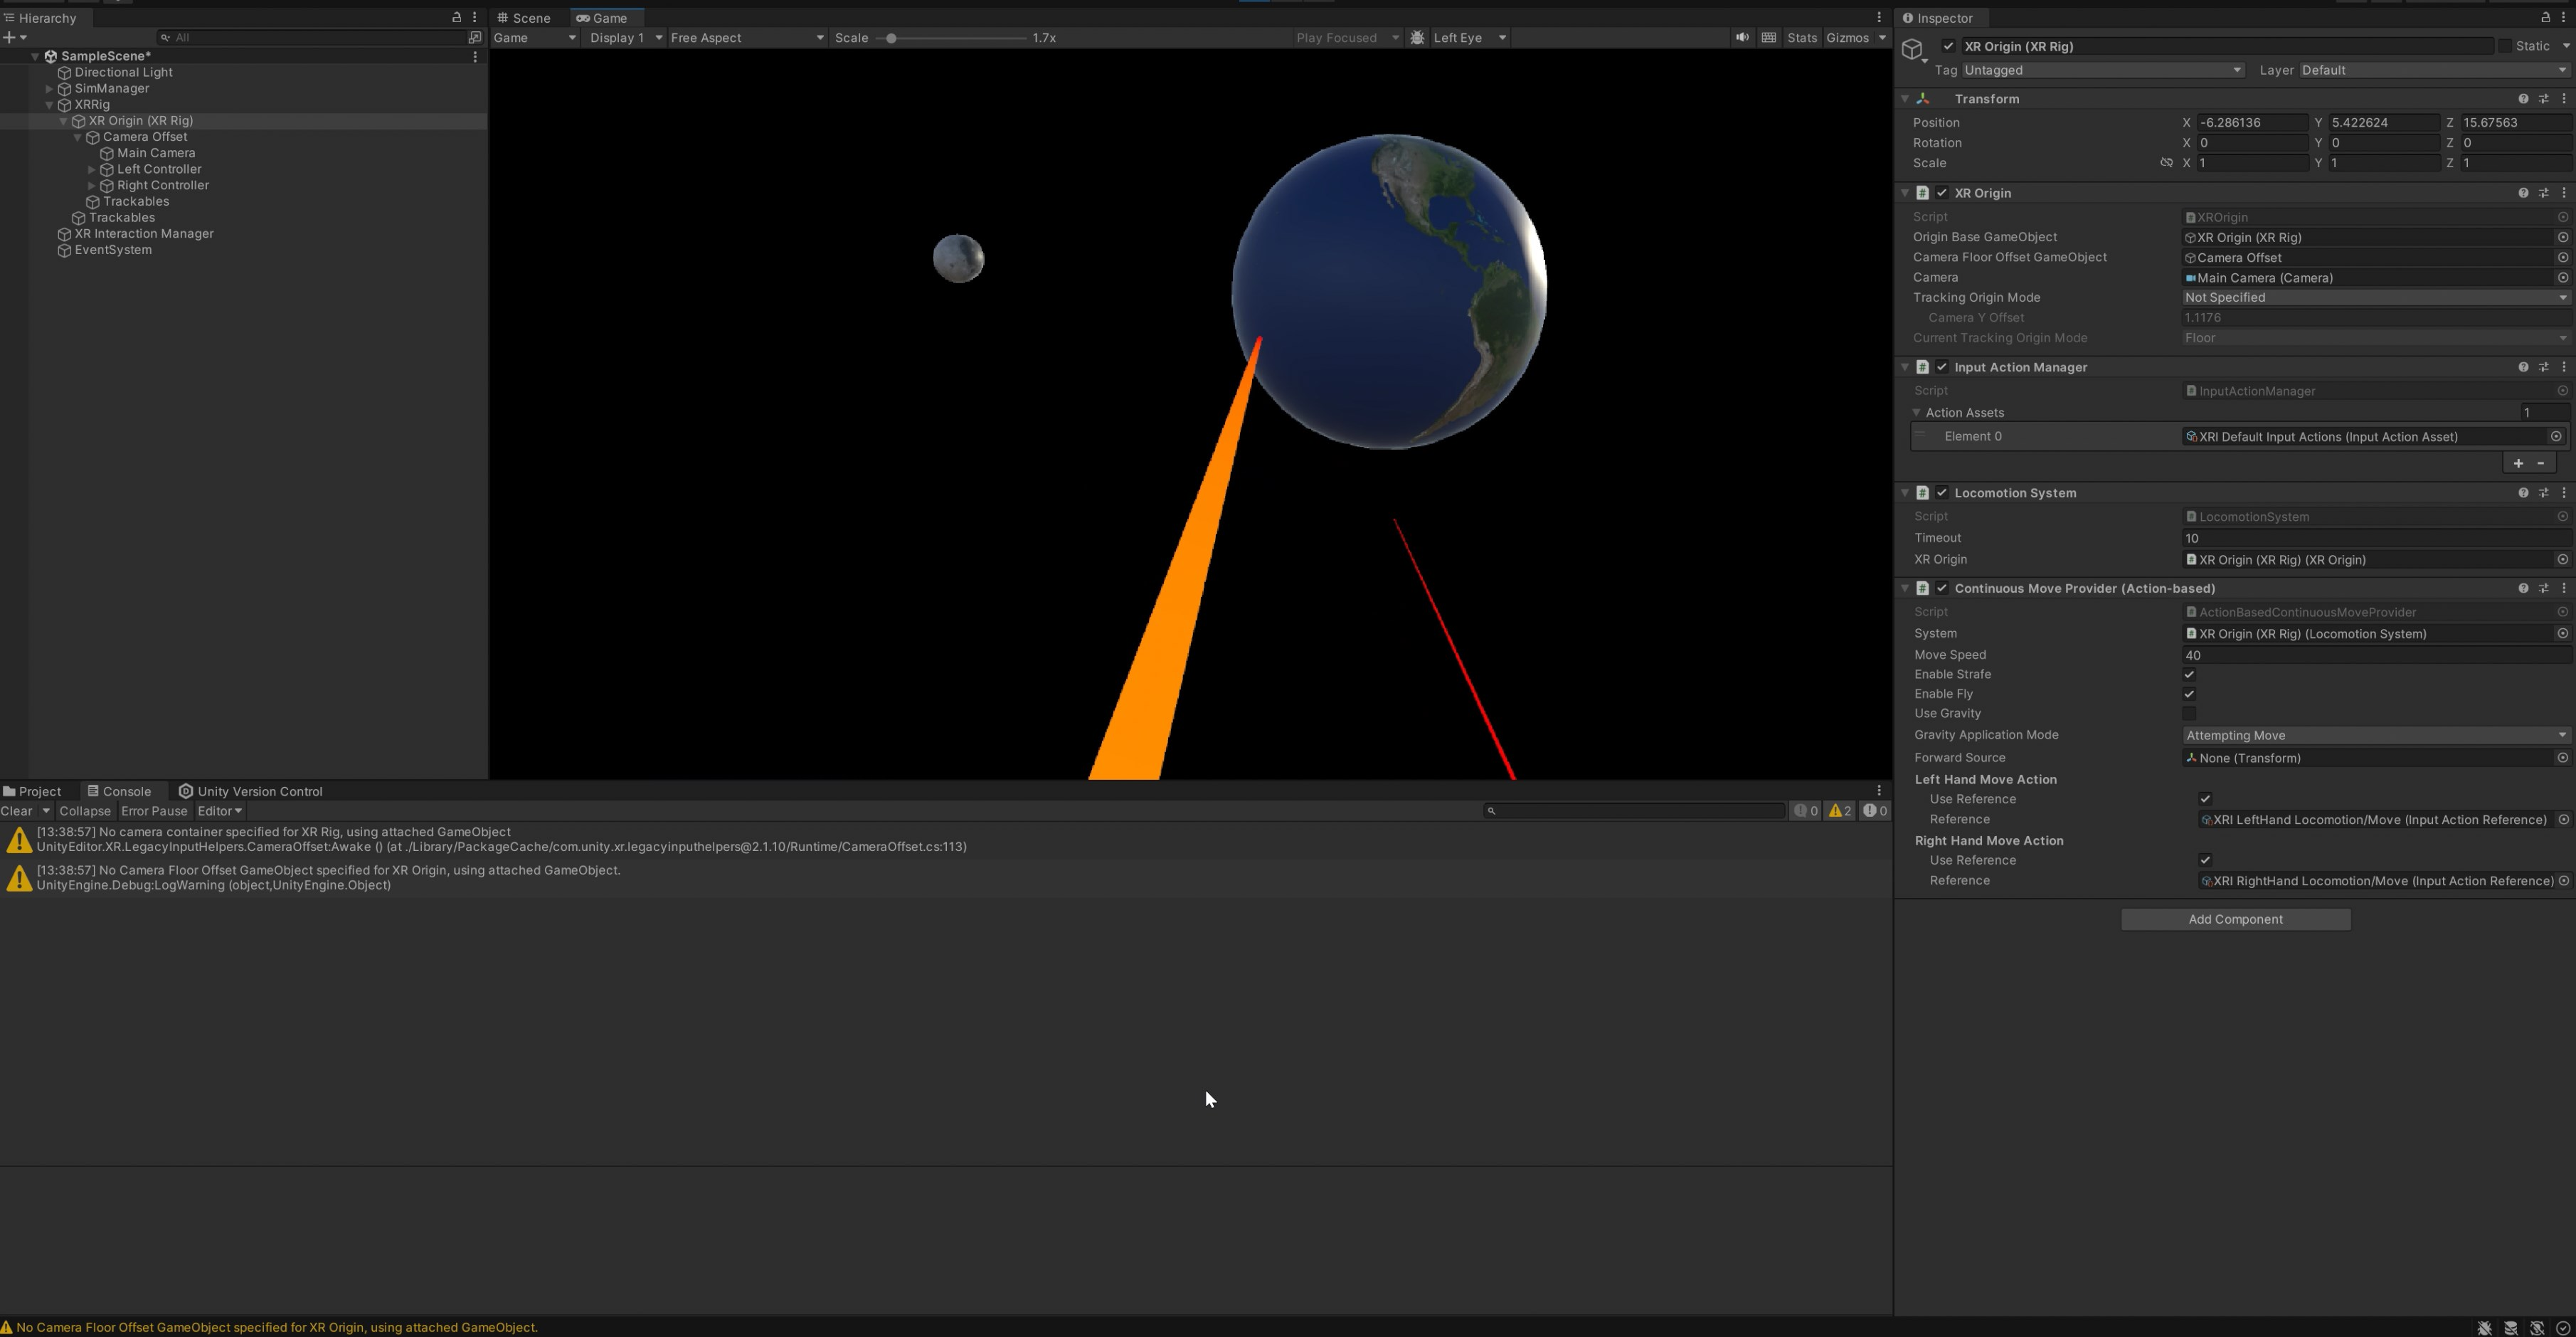
\includegraphics[scale=0.25]{vr_test1.jpg}
        \caption{Initial VR test of the simulation.}
        \label{initialvr}
    \end{figure}
    \section{Instructions}
    The camera can be moved by using the W, A, S, and D keys on the keyboard, and can be panned to look around by moving the mouse (see figure \ref{keyboard} and figure \ref{mouse}). In VR (on an Oculus touch controller), the left analog stick is used for continuous movement. Camera panning is of course done by looking around while wearing the HMD. Keyboard and mouse input will be disabled when playing the simulation in VR.
    \begin{figure}[h]
        \centering
        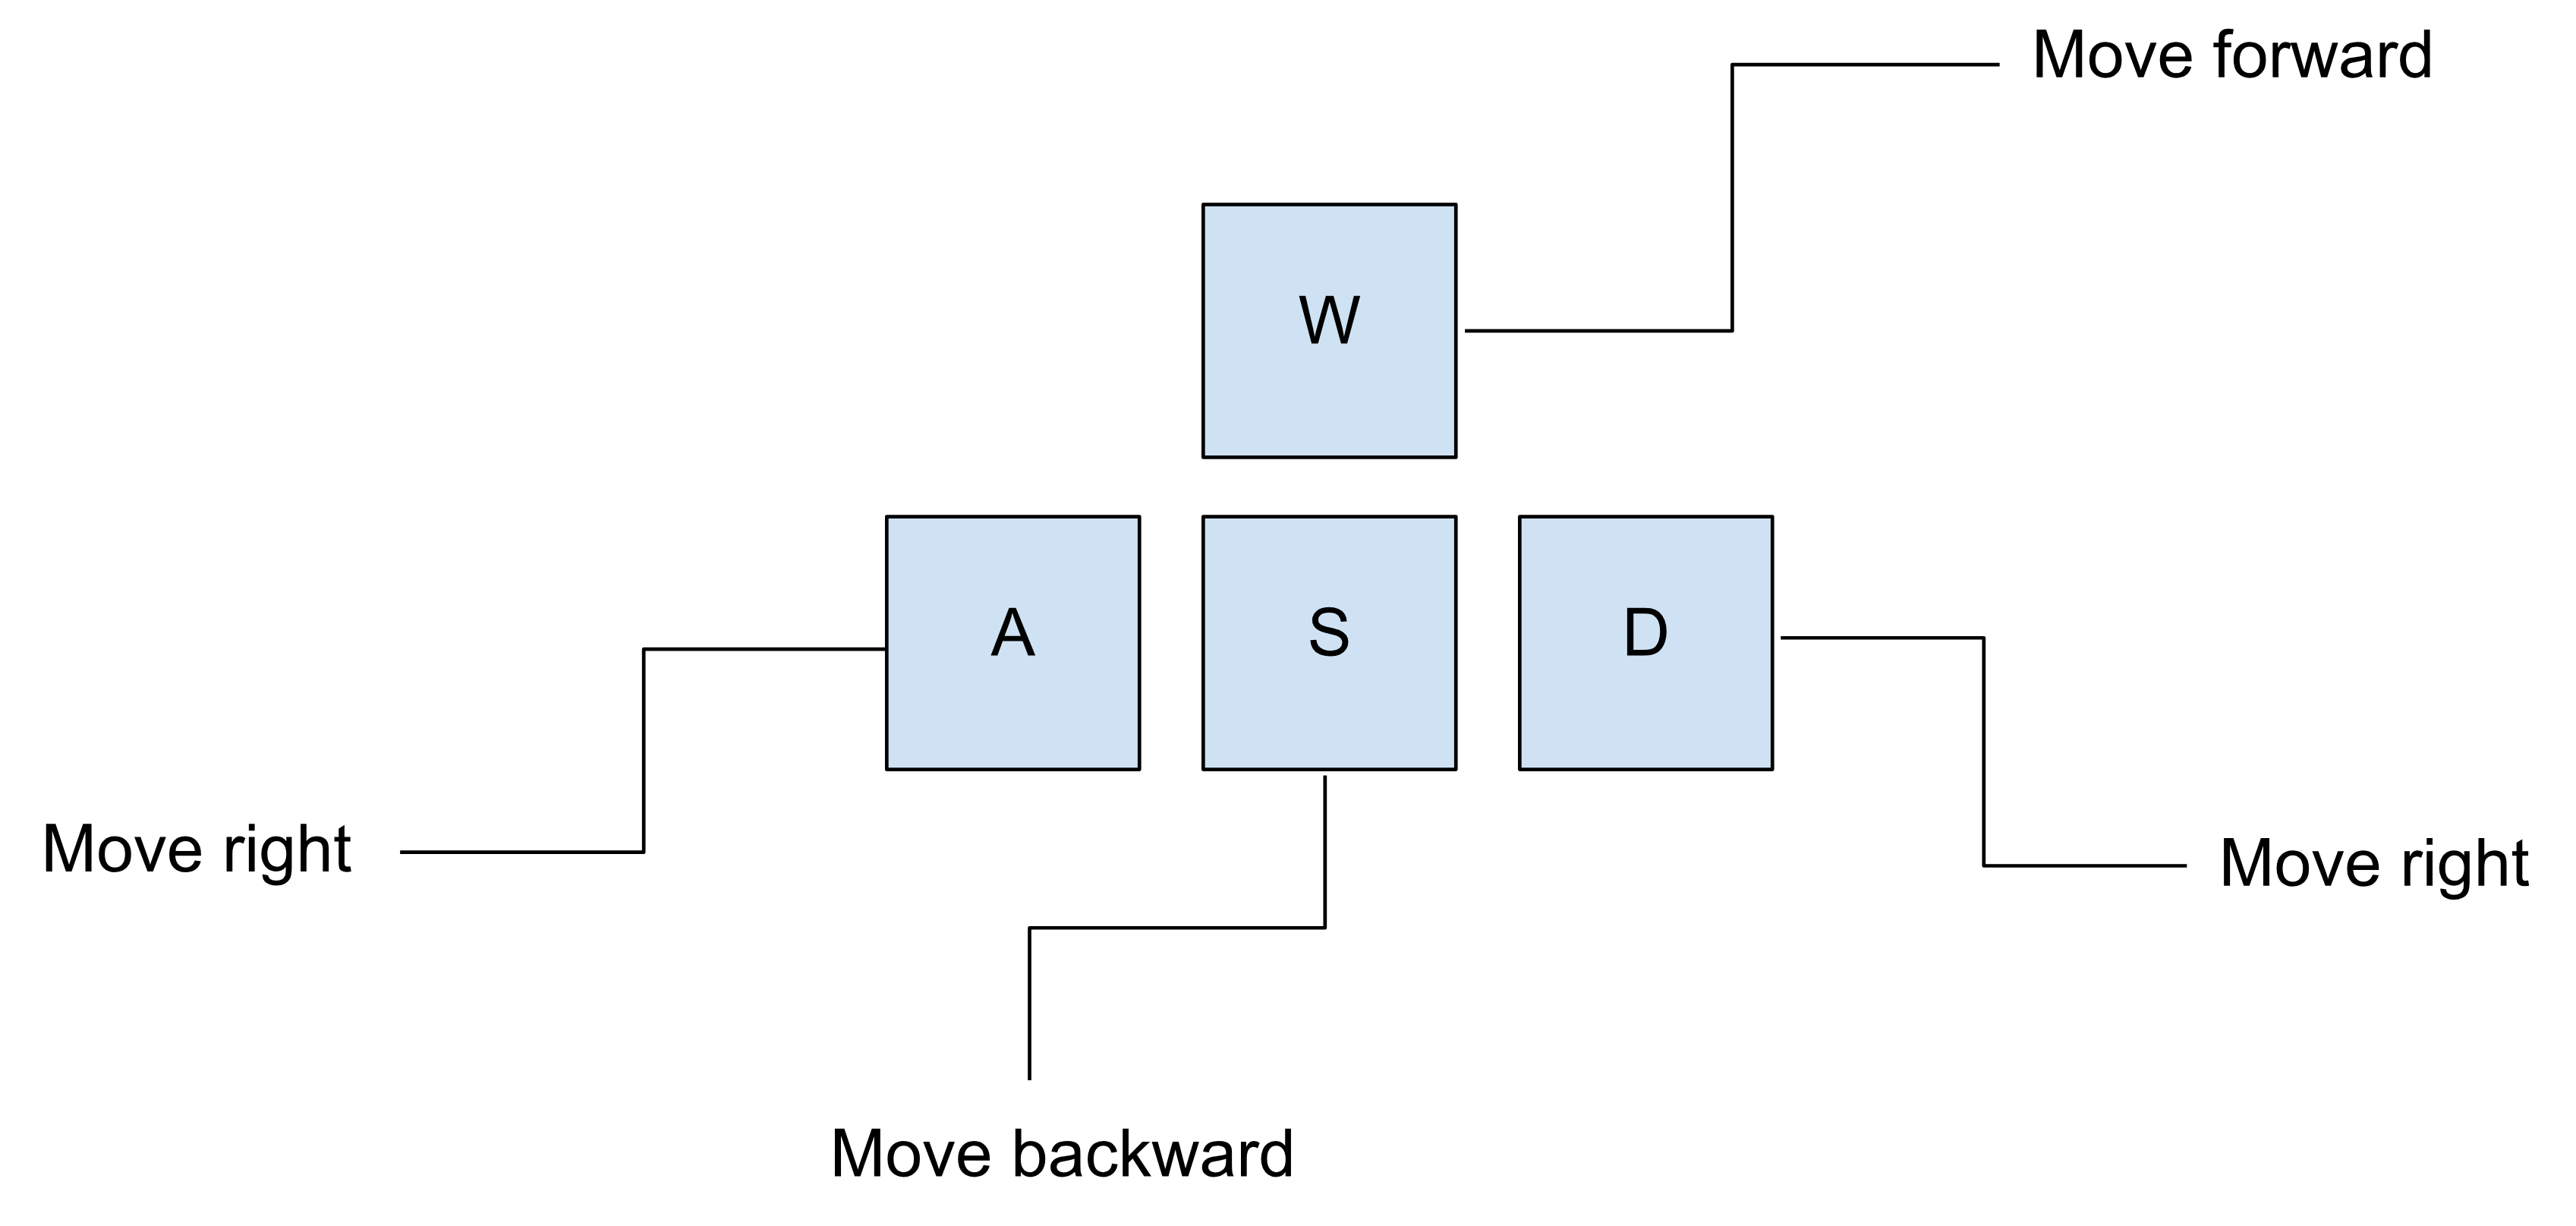
\includegraphics[scale=0.2]{keyboard_controls.png}
        \caption{Keyboard controls.}
        \label{keyboard}
    \end{figure}
    \begin{figure}[h]
        \centering
        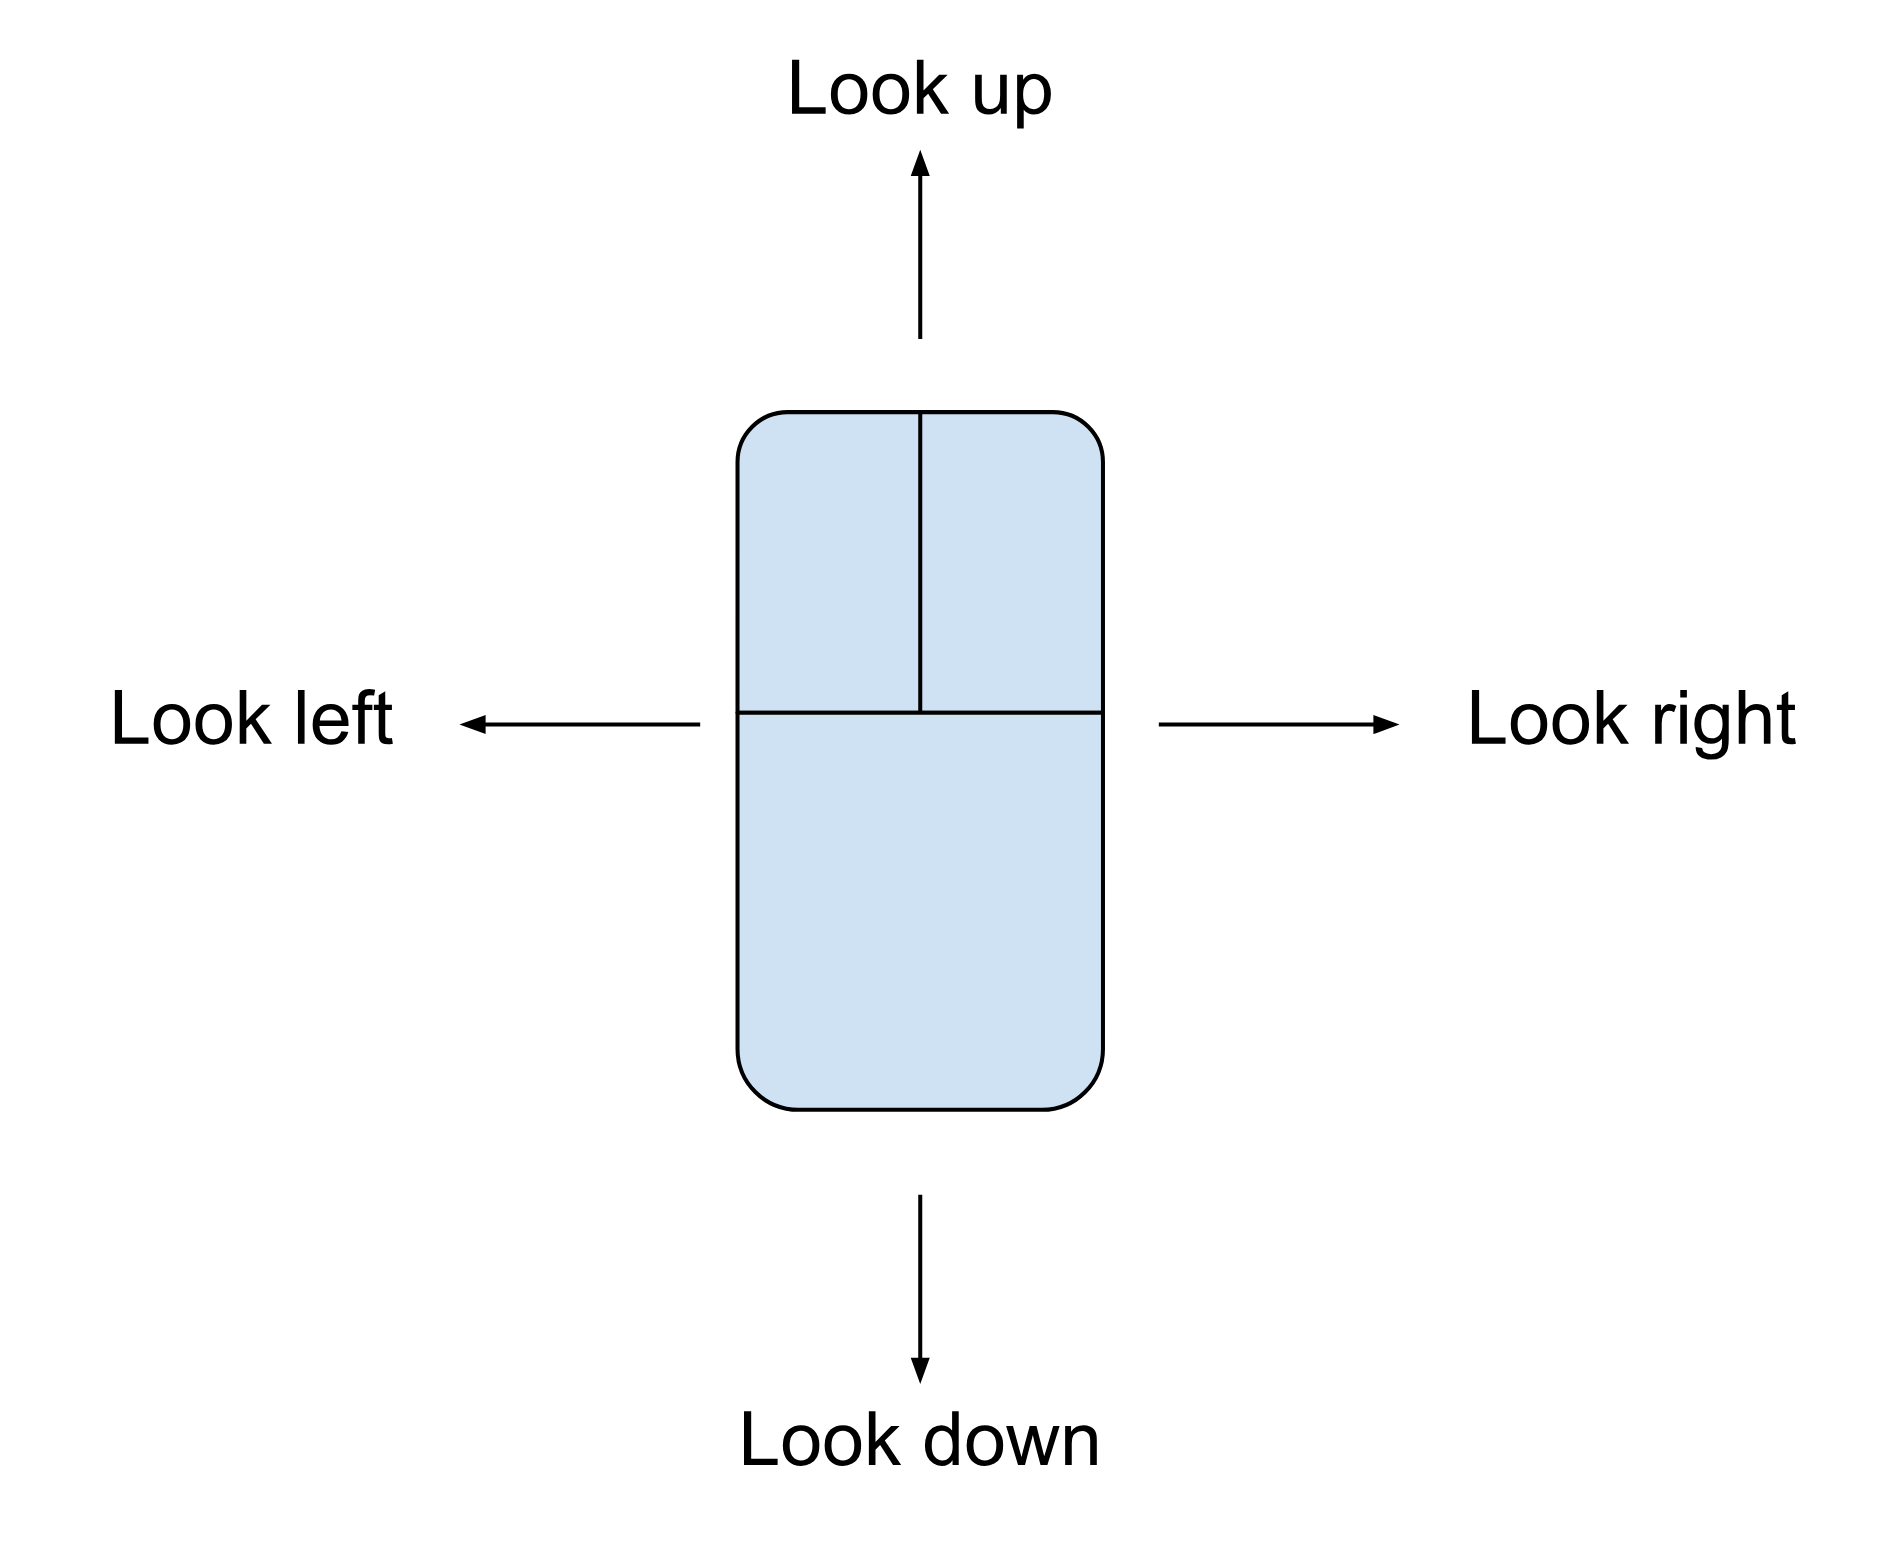
\includegraphics[scale=0.25]{mouse_controls.png}
        \caption{Mouse controls.}
        \label{mouse}
    \end{figure}
    \section{Considerations}
    To reduce the scope of this project, only the Earth's moon will be simulated. Including moons from all other planets is unnecessary for what is trying to be shown in this simulation. To enhance the visual appeal of the simulation, random asteroids will spawn and be simulated. These asteroids have no consequences on the rest of the simulation however as they will not interact with any of the planets in any meaningful way.
    \section{Challenges}
    The built in Unity physics engine was not very well suited for the simulation of planetary motion, and thus was replaced with a custom solution. The Unity physics engine is a good fit for games that usually take place in some world with Earth-like gravity, but it does not offer any functionality for simulating planetary motion.

    For project collaboration, Unity Cloud was considered, but it is only free for the first 3 seats. For this reason, we chose to use git with GitHub for source control instead.

    Another point of issue during development was converting an existing Unity project to one that supports XR. While it should be very simple in theory, the Unity documentation for the version of Unity used in this project was slightly incorrect. This lead to an extended amount of time being spent trying to debug the wrong problem. The Unity documentation points to the documentation for version 3.0.3 of the ``XR Interaction Toolkit''. However, when attempting to use the Unity package manager, it claims that the latest version is 2.6.3. These two versions are completely incompatible and have different APIs. For some reason, the VR sample project uses version 3.0.3 (on the same version of Unity!), but the Unity package manager will not install it in an existing project.
    \newpage
    \bibliographystyle{IEEEtran}
    \bibliography{refs}
\end{document}
